This chapter covers the evaluation of the master's thesis. The goal of the evaluation is to assess the suitability of ChatGPT in performing  different steps of the refactoring pipeline, and whether such refactoring is accepted.



The evaluation is split into two distinct experiments that use two different methodologies. Figure \ref{fig:exp_comparison} shows the general methodologies of both experiments. 

\begin{figure}[ht!]
    \centering
   \begin{subfigure}[t]{0.49\columnwidth}
   \centering
    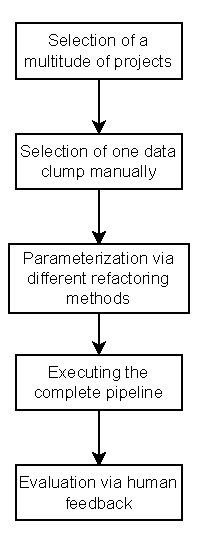
\includegraphics[]{figures/chapter5/evalPartASequence.drawio.pdf}
    \caption{Experiment 1:\\
    feedback-based evaluation}
    \label{fig:exp1_sequence}
    \end{subfigure}
     \begin{subfigure}[t]{0.49\columnwidth}
     \centering
        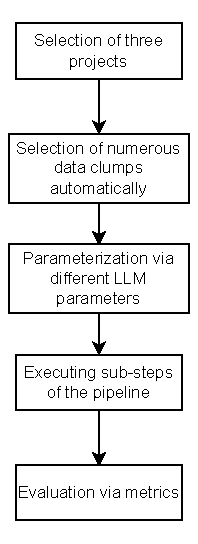
\includegraphics[]{figures/chapter5/evalPartBSequence.drawio.pdf}
        \caption{Experiment 2:\\ metric-based evaluation}
        \label{fig:exp2_sequence}
    \end{subfigure}
    \caption{Flowcharts comparing both experiments}
    \label{fig:exp_comparison}
\end{figure}

In section \ref{sec:pull_request_eval} the  first experiment is discussed.  This experiments attempts to answer RQ 1 about the acceptance of \ac{LLM}-assisted refactoring. 

As figure \ref{fig:exp1_sequence} outlines, several GitHub projects are selected.  In each of these projects, one data clump is selected manually. This data clump is refactored via the tool. The experiment is parameterized via two different refactoring methods. In one experimental setting, the \ac{LLM} only proposes a suitable name for the extracted class but the refactoring is performed via the \ac{PSI}  while in the other setting the refactoring is performed by the \ac{LLM} alone. The experiment is evaluated by submitting \acp{PR} via GitHub and asking for feedback from contributors of the selected projects. 



The two remaining research questions about the potential of \acp{LLM} in the refactoring pipeline are handled in section \ref{sec:metric_based_eval}.

 As the flowchart in figure \ref{fig:exp2_sequence} shows, there are key differences. Only three projects are selected. However, more data clumps are chosen. This time, data clumps are selected automatically (e.~g. randomly or via metrics). Additionally, a larger set of parameters is varied. Moreover, the focus on this experiment is not to test whether the tool can successfully execute the complete refactoring pipeline but subsets of it. For instance, it is tested whether the \ac{LLM} can filter data clumps given that data clumps have already been detected. In contrast, to the first experiment, no human feedback is sought but different metrics are used that attempt to evaluate the performance of \acp{LLM}. 


These two experiments complement each other and help to assess the potential of \acp{LLM} in the refactoring pipeline. 
Studies have shown that traditional metrics like cohesion or coupling are insufficient to provide information about software quality \cite{search_based_refactoring}.  However,  a feedback-based based approach (e.~g. via interviews or surveys) is more time- and resource-consuming so that it is often  not used to validate refactoring tools. Additionally, feedback-based evaluation  requires experience  in the respective development area. \cite{automatic_software_refactoring_literature_review}

Hence,  two-sided evaluation approach integrates both human feedback and systematic analysis to provide a comprehensive understanding of the tool's efficacy and applicability.
As both experiments have their potentials and challenges, it can be useful to perform these distinct experiments to evaluate the potential of ChatGPT in the data clump refactoring pipeline.












\section{Experiment 1: Pull request evaluation}\label{sec:pull_request_eval}
In this section, the first evaluation about pull requests  related to data clump refactoring is discussed. 

To ascertain the quality of refactoring, human feedback is essential \cite{search_based_refactoring}. While there are metrics to evaluate whether a given refactoring is useful, the metrics do not always align with the viewpoints of developers. 

 For example, the \textit{DataClumpDoctor} tool might identify data clumps that not all developers would agree are problematic. Discrepancies might arise over the minimal number of data clump items (three in this master thesis). Additionally, developers who are  familiar with the projects's structure may more accurately judge  whether a group of variables  is worth refactoring. In some cases, they have written the method or class themselves and have introduced the data clump on purpose. One reason for this decision could be that they were unable to find a proper name for the extracted class, or the disadvantages discussed in section \ref{sec:data_clump_not_refactor} outweigh the advantages of removing data clumps.

Even if developers see that refactoring a data clumps could be helpful, there could be arguments against refactoring them. These reasons include the points  discussed in section \ref{sec:data_clump_not_refactor}. However, there could also be other reasons that apply to code smells in generals. For instance, developers might combine refactoring with the introduction of new features, rather than refactor solely for its own sake. 

As a result, collecting  the opinions and insights of developers on whether data clump refactoring is justified and can be performed by a \ac{LLM}  forms the foundation of this evaluation.





\subsection{Methodology}

Figure \ref{fig:flowchart_expA} shows the general methodology of the first experiment. 
In this experiment, GitHub projects were selected to refactor a single selected data clump via a pull request and feedback was collected from contributors of the projects to ascertain the refactoring quality of ChatGPT. 


\begin{figure}[ht!]
    \centering
    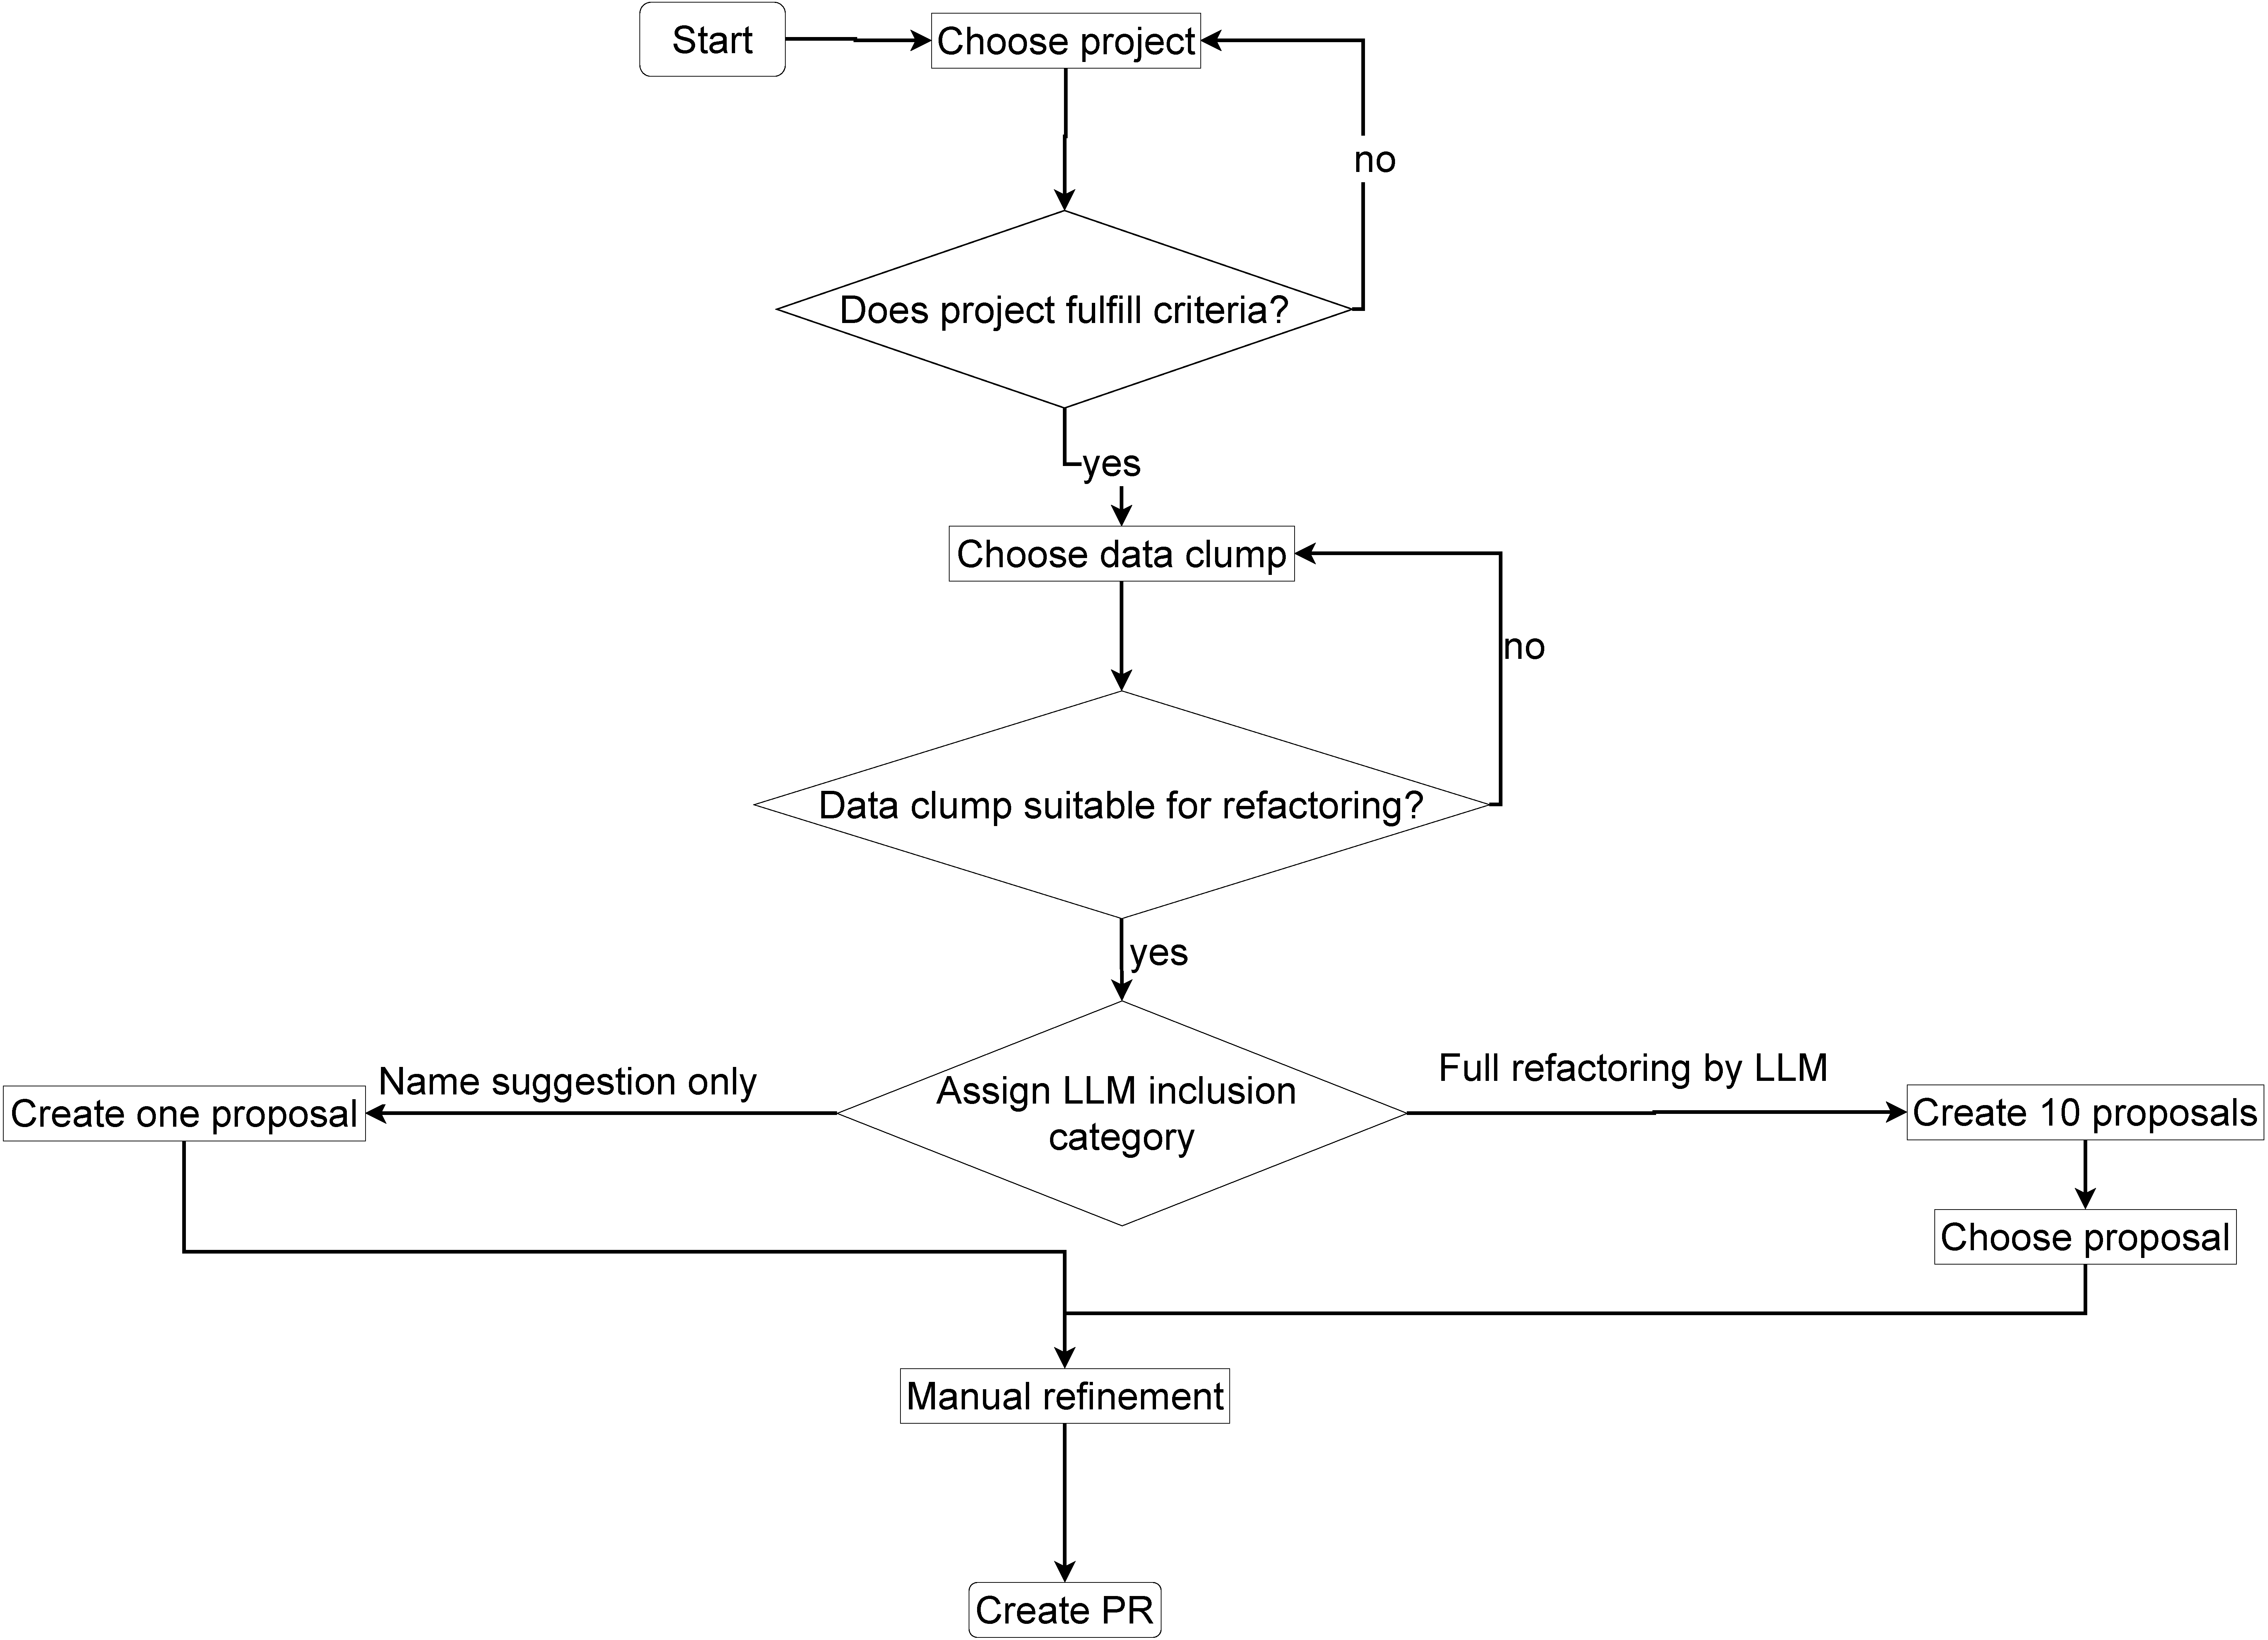
\includegraphics[width=1\columnwidth]{figures/chapter5/flowchart_expA.drawio.pdf}
    \caption{Methodology of the first experiment}
    \label{fig:flowchart_expA}
\end{figure}

\subsubsection{GitHub project selection}\label{sec:github_projects}

To facilitate the evaluation, GitHub projects are selected to be analyzed in the first experiment. 


The projects were selected from the trending page of GitHub. This page list GitHub projects that have gained significant attention over a specific  period. While the exact criteria for this listing is not disclosed, popular indicators include higher-than-average forks and stars.

To ensure a sufficient number of data clumps, only larger projects were considered. This increases heuristically the chance of having a higher number of data clumps, and also the chance of getting more developers to respond to the survey as larger projects tend to be maintained by more people. 

Since active participation of developers was necessary for the survey to work, only process with recent activity are selected. Only if pull requests are frequently considered and closed (which does not necessarily mean that they are merged), the project was considered active enough. 

In addition, the project had to be able to build without flaws. This ensures that the eventual refactoring can be evaluated smoothly. If the project did not compile properly or tests were failing, it became more difficult to determine whether these errors were caused by a refactoring or whether they existed from the beginning. This would be an obstacle to the manual refinement step.

%As a result, it was beneficial to make sure that these projects do build correctly. This can be checked by executing \textit{mvn clean package} or \textit{gradle clean build} (depending on the build system) as these commands usually run all required tests.

Hence, each selected project must comply with the following criteria:
\begin{enumerate}
    \item The project contains at least  10,000 \ac{LOC} of Java
        \item The project  has at least 100 stars
\item Any pull requests have been merged in the last 30 days
\item The project compiles and all tests run flawlessly.
\end{enumerate}


The total number of projects and hence pull requests was not predetermined at the beginning of the experiment. The goal was to create as many pull requests as possible. 


\subsubsection{Guidelines for selecting data clumps}

For each selected project, one data clump was chosen. To initialize this data clump selection process, the metrics described in section \ref{sec:data_clump_filtering} were combined. These metrics include the occurrence, size, and affected files metric. The top ten most-scored data clumps were manually reviewed to determine a data clump for refactoring. The selection process was supported by:
\begin{itemize}
\item A proposal by ChatGPT. 
    \item Any filter discussed in section \ref{sec:data_clump_filtering} would trigger (e.~g. abstract class, generics, annotations).
    \item The data clump items share a common domain such that extracting a class is useful. 
    \item The project is a library used by other programs so that refactoring of public or protected components should be carefully scrutinized. 
\end{itemize}

\subsubsection{LLM inclusion category}

After considering all of these criteria, one final data clump was selected.
After a data clump is selected, the next step is to assign the project to one of two categories to determine the extent \acs{LLM} are used to find and refactor data clumps. 



In the first category, ChatGPT performs the refactoring alone. Because transmitting whole GitHub projects would infeasible, the \textit{DataClumpDoctor} was used to detect the previously selected data clump and obtain all locations of interests. A margin of 5 was used so that 5 lines below and 5 lines above each location of interest were transmitted. 

Then, ChatGPT is instructed to refactor the data clump in the provided locations of interest. This instruction was repeated at least ten times, in each time the context of ChatGPT was cleared so it didn't know its previous answers. 

From these ten proposals, one proposal was chosen that describes refactoring data clumps most accurately. For instance, the extracted class is valid, most usages of the data clump items are updated and all method signatures are refactored (if applicable). Generating multiple proposals is necessary because not every proposal would be correct. 



The second approach for refactoring was via IntelliJ. In this case, ChatGPT only suggests a suitable name for the extracted class but is otherwise not involved in the refactoring. Instead, the \ac{PSI} performs all refactoring in the manner described in section  \ref{sec:intellij_refactoring}. This results in a very consistent refactoring without any creativity. Hence, this refactoring needs only to be executed once and the first proposal can be selected immediately. 

\subsubsection{Manual refinement}

After selecting a proposal, the proposal is applied and saved on a separate branch.
Afterwards, the proposal might not be fully correct. For instance, there might be  none-updated method calls, missing semicolons etc. An additional problem occurs if code style tools like \textit{SpotBugs} or \textit{Checkstyle} are employed. If the refactoring by the \ac{LLM} does not conform to the required codestyle, the code might not compile because the developers of the project force a certain style. Therefore, a manual correction step is performed. The project is  manually changed in such a way that it fully compiles. However, no creative refactoring is performed. For instance, if one part of the source code was not refactored, it was refactored like another part regardless of whether another refactoring might have made more sense. This reduces human intervention to a minimum and ensures that the creative part of the refactoring is done by the \ac{LLM}. 

\subsubsection{PR creation}
As soon as this manual refactoring finished and the program compiles, the changes were squashed into one commit and a pull request was created in the respective repository.

 A pull request is a proposal by a contributor to change some parts of the source code in a GitHub project. These changes can relate to fixing bugs, introducing new features or refactoring the code base. The proposals can be discussed and amended so that the proposal can be improved. By using continuous integration and continuous deployment, the changes can be tested automatically. Only if the changes are acceptable to an integrator (e.~g. the owner of the GitHub project), the changes are merged into the project. If not, the pull request can be closed without further consequences. \cite{pr_decisions}

In the pull request of the experiment, the maintainers were described the purpose of this pull request and  the definition of data clumps used in this master thesis. They were asked to give feedback by filling out a feedback form or by giving feedback via GitHub comments under the respective pull request. It was explicitly stressed that rejecting the pull request would not be perceived negatively. The full text of the pull request can be found in appendix \ref{app:pr_text}.

\subsubsection{Feedback survey}\label{sec:feedback_survey}

Feedback was collected from two sources that were available on each pull request. 

One  natural way of providing feedback over GitHub is via comments. These comment can be review comments that address specific parts of the code, or general comments unrelated to any code that addresses the pull request as a whole. \cite{10.1145/3597208}. Therefore it is an important source of determining the acceptance of the proposed refactoring. However, since the comments are natural texts, the evaluation is more challenging.


On the other hand, surveys commonly use the Likert scale, which presents statements and asks respondents to choose a response from discrete attitude categories. \cite{edmondson2005likert}
For instance, a statement might be \enquote{Data clumps are a code smell that should be fixed} and a respondent could choose between \enquote{Agree}, \enquote{Neutral} or \enquote{Disagree} for this statement. 


The topics of the survey  ranged from the usability of \acp{LLM} in software engineering, to the quality of the proposed refactoring, and the experience of the respondents. 


Details about the survey can be found in appendix \ref{app:pr_survey}


\subsubsection{Evaluation metrics}

For the evaluation, the following metrics are used:
\begin{itemize}

    \item  How many PRs are merged or rejected.
    \item The numerical value of the likert scale.
    \item Topics mentioned in the comments that are either positive or negative. For instance, a comment might mention that the readability is improved or worsened by a refactoring. The occurrence of these topics can be counted.   Table \ref{tbl:feedback_categories} explains the most important feedback categories. 

\end{itemize}

By grouping the pull requests into categories (e.~g. by refactoring method, data clump type etc.), these metrics can be used to gather hindsight into the acceptance of \ac{LLM}-assisted refactoring. 

To evaluate this experiment, the null hypothesis \enquote{Developers do not accept data clump refactoring via \ac{LLM}} is presumed. This null hypothesis is rejected if \textbf{all} of the following conditions are met:

\begin{enumerate}
    \item At least 20~\% of the pull requests are merged
    \item The median Likert score for each of the survey questions is at least \enquote{Agree} (or 3 numerically)
\end{enumerate}

The first criteria takes into account that even good pull requests can be rejected for any reason so that a high threshold would not be helpful. The second criteria measures the acceptance of the PR. The feedback via text comments is left out as it would be difficult to describe a criteria by which the null hypothesis might be rejected.

Only if the developers generally agree with the changes by the pull request, the null hypothesis can be rejected with confidence. 


\begin{table}
\begin{tabular}{p{4cm}|p{10cm}}
	Comment & Description\\\hline
	\textit{Refactoring not worth it} & The refactoring does not provide enough advantages to justify it\\\hline
	\textit{Readability} & The readability of the source code is reduced \\\hline
	\textit{Not enough} & While the refactoring could be a good idea, more changes should be performed to make the refactoring more useful \\\hline
	\textit{Intentional design choice} & The duplication of variables is warranted so that changes are unnecessary \\\hline
	\textit{Style adaption} & The refactored code does not fit into the rest of the code as it violates style guidelines. \\\hline
	\textit{Complexity} & The refactoring introduces more complexity\\\hline
	\textit{Semantic changes} &  The refactoring changes the semantic of the code\\\hline
	\textit{Performance}& The performance implications of the refactoring are too grave \\\hline
	\textit{Java record better} & The extracted class suggested by the refactoring could be converted into a Java record \\\hline
	\textit{Extracted class should not be public} & Instead of creating a new file for an extracted class, it should be located inside another class and does not need to be public \\\hline
	
\end{tabular}
\caption{Feedback categories explained}
\label{tbl:feedback_categories}
\end{table} 




\subsubsection{Ethical consideration}
As this survey contains interaction with human-beings, a small analysis on the ethical implications is conducted. Several precautions are undertaken to address any possible ethical concern. 

First of all, full transparency is provided  with regard to the pull request. The pull request message explicitly states the purpose of the PR as a part of a scientific project. Also the use of an \ac{LLM} is explicitly stressed so that no misunderstanding can occur. However, the participants are not aware of the extent \acp{LLM} have been used and do not know which model was used. Such details have however been revealed during discussion of the PR if further feedback from new participants was unlikely.

Additionally, the requests were not sent en masse but after careful consideration. Only if it is thought that a pull request does compile, passes all unit tests and otherwise does not have major issues, the pull request is submitted. Of course, mistakes can happen so that this approach cannot guarantee hundred percent fault-free code. Since many projects needs to be considered, the extensive knowledge of the software project, which a regular contributor has, is missing, so that the chance of faults is higher. Nevertheless, pull requests can be created by anyone and the review process by continuous integration and deployment tools and human beings is a safeguard to limit the risk of faulty code added to the code base. 

Last but not least, it was attempted to minimize the burden on the reviewers. For instance, data clumps affecting a significant number of files were not refactored. Also only one pull request per project was created, thereby minimizing the chance that a participant might review multiple pull requests. 

At one instance, an ethical complaint was filled because of the use of \acp{LLM} and the perceived spamming of pull requests. This complaint was however dismissed by the responsible organizations of the University of Osnabrück.


\subsection{Results}

At the conclusion of this experiment, pull requests to 40 projects were submitted. Of those 40 projects,  feedback for 31 projects could be obtained. In the remaining 9 cases, either the pull request is still open, was closed without meaningful feedback or merged without meaningful feedback. In 8 cases, the pull request was eventually merged which indicates a acceptance rate of twenty percent. 

In 7 projects, feedback was provided via the survey. 8 comments were received via the survey which means that for one project the survey was filled out twice. Figure \ref{fig:boxplot_survey} shows the result of the evaluation if only the Likert scores are considered. 

The box plot shows that developers have a weak tendency to consider data clumps as a code smell worthy to fix as the median is about 2.5 (neutral to agree). Since the lower whisker shows a value of 1, it can be assumed that there is some disagreement about this code smell.

The statement that \acp{LLM} are useful receives more agreement. There is one outlier that has a neutral altitude whereas all other Likert values shows agreement or strong agreement. 

There is significant opposition to the claim that the proposed refactoring improves the source code. The median lies at 1 which indicates disagreement. 

With regard to the preservation of functionality, the respondents generally agree that the functionality is remains as before. One outlier exists. In that particular case, the handling of the \textit{NonNull} annotation is not preserved which the respondent sees as a disadvantage. 

As significant variance exists for the claim of the suitability of the chosen name for the extracted class. While the median is at 3, there is a wide range of different answers to this statement which indicate that the selected names are not always liked. 

On the other hand, there is less opposition for the location of the new class although the outlier show that the selection of the location still poses some challenges. 

As a result, while the first rejection condition of the null hypothesis is met, the second fails. Therefore, the null hypothesis fails to reject. This means that the first RQ \enquote{Do developers accept data clump refactoring via ChatGPT?} cannot be answered positively.

\bigskip
\begin{figure}
    \centering
    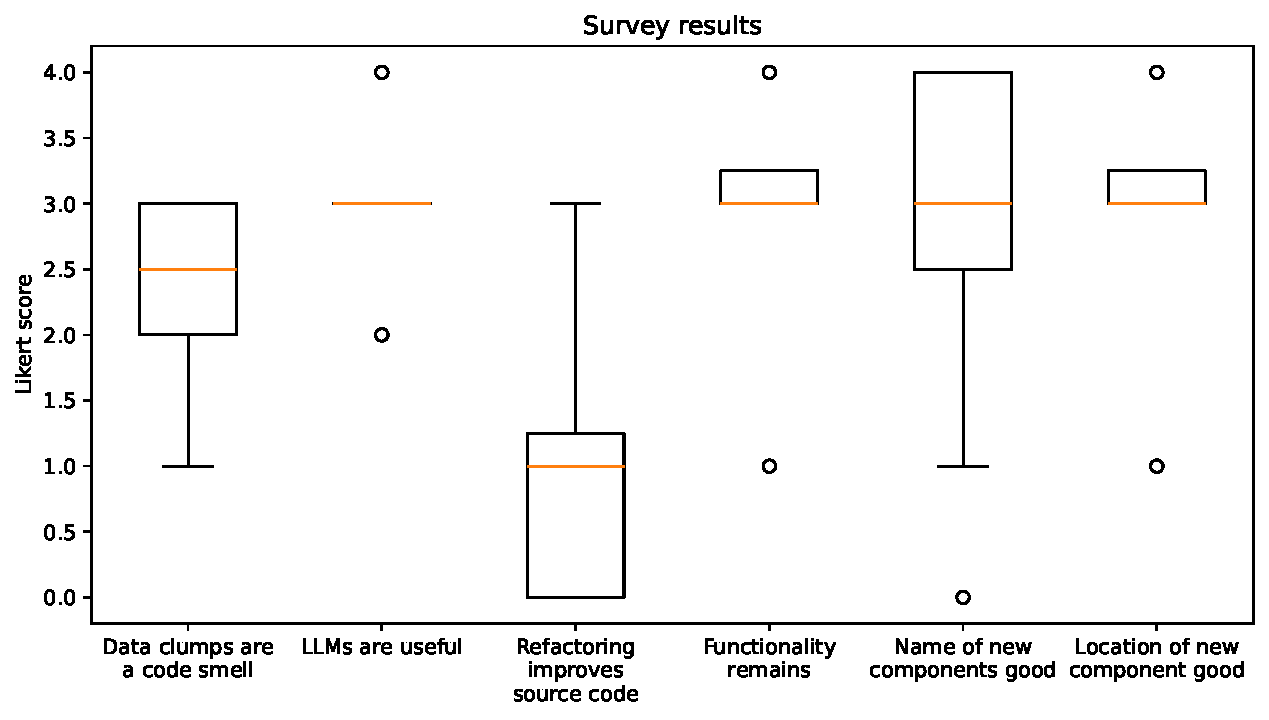
\includegraphics[width=\columnwidth]{figures/chapter5/survey_results.pdf}
    \caption{Boxplot of Likert score from survey}
    \label{fig:boxplot_survey}
\end{figure}


The textual feedback contains further hindsight on why the refactoring was perceived more negatively. In six instances, the reviewers perceived an increase of complexity. In 11 instances, there were concerns about the readability. Also, performance concerns were common as the refactoring entailed creating new instances. This criticism was shared five times. Another argument that was made nine times is that the refactoring was not worth it as the developers see no obvious benefit in refactoring this data clump.

The difference of the feedback between the traditional refactoring and the \ac{LLM}-driven refactoring is slim. However, there are noteworthy observations. For instance, the traditional approach receives four instances where the maintainers are dissatisfied with the style adaptation of  the code. This means that the refactored code did not fit into the rest of the code. This point was not risen for the fully \ac{LLM}-generated code. 

Also, in general, criticism about the code readability was raised more for the project refactored using the traditional approach than the \ac{LLM}-based approach.

Comparing the refactoring of fields-to-fields to parameters-to-parameters data clump, there are also some differences. The readability of refactored fields-to-fields data clump was  scored more negatively than that of parameters-to-parameters data clump. Also the adoption of the code to the style was criticized more if fields-to-fields data clump were refactored. Additionally, more meaningful comments were received for parameters-to-parameters data clump.

Noteworthy, the refactoring performed by the model had not always refactored an actual data clump as defined in section \ref{sec:data_clump_def}. In one case, a group of fields that only existed in one class but have a semantic relationship were extracted to a class. Nevertheless, this pull request was merged indicating that a close semantic connection of variables can warrant refactoring. However, in two other similar cases, the pull request was rejected. 

The occurrence of a data clump strongly influences the likelihood of a refactoring being merged. Refactorings that were not merged had a mean occurrence of 4.5, whereas those that were merged had a mean occurrence of 10.7

If one considers the size of the refactored data clump, there are also some patterns. For instance, the respondents believe that larger data clumps reduce the complexity. However, on the other hand, the readability of the refactored source ode was higher if the data clump is smaller.

\subsection{Threats to validity}

The survey evaluation has some threats to its validity that should not be disregarded.

To begin with, the selection of GitHub projects was not completely unbiased. For instance, currently trending GitHub projects were chosen although it is not certain why they were popular. Therefore, the maintainers of the project might not be fully prepared to deal with associated surge in pull requests associated with trending projects. This can increase the chance that a pull request (even though reasonable and well-meant) is summarily rejected. \cite{10.1145/3366423.3380272}

Additionally, only projects that do build flawlessly were considered. Usually, this should be case for every project, but the reality differs. For instance, the operating system, the installed libraries, the Java version, and other components can have a significant impact on whether all unit tests complete without errors and the project builds.  While every effort was made to give each project a chance to compile, at some point, time constraints prevented endless consideration of a project. Hence, if even after testing on multiple system, reading the associated documentation, and testing multiple Java version, no fully functional build was achieved, the project was disregarded.

It is also important to consider the manual correction process, as it could introduce mistakes or bugs due to human error rather than errors from the \ac{LLM}. Feedback regarding these errors must be filtered out as they are not relevant. This manual correction process can also shift the quality of the refactoring upwards so that the respondent would rate the raw PR more negatively. 


Additionally, the decision to accept or reject a pull request can depend on many factors. For instance, the current mood of participating developers can influence the rejection rate \cite{detecting_emotional}.

For larger project, bureaucracy was also a factor that prevented the creation of pull requests. For instance, some projects require that pull request must always relate to an existing issue so that the general idea can be discussed without providing source code. For usual contributors, this might be beneficial as they do not need to spend time on writing code that is rejected in the end because the developers do not like the general approach. For the purpose of this evaluation, the actual source generated is essential, so creating an issue first would be possible,  but more burdensome  and would not add much value. Nevertheless, the sole existence of such rules was not a criterion to filter out a project. 

Furthermore, using a survey with the Likert scale can lead to problems since such an analysis can have its flaws as it implies that the distance between response categories is constant. For example, it might be easier or harder to choose between \enquote{Strongly Disagree} and \enquote{Disagree} compared to \enquote{Strongly Agree} and \enquote{Agree} \cite{HARPE2015836}.

As the results show, participation in the survey is essential. Because only seven developers responded to the survey, the results can only be taken with a grain of salt. The small sample size also means that the interpretation of the median and other statistical metrics is less meaningful.

\subsection{Discussion}

One main finding on the evaluation results is the importance of selecting suitable data clumps for refactoring. In many cases, the developers believe that the suggested refactoring is not worth it, makes the code harder to read or the performance implication are too negative. This shows that data clumps are a code smell where there is a wide disagreement on when refactoring is warranted and when not. because all tested projects have a multitude of different data clumps that have various sizes, affected files or included variables, it is very difficult to select a suitable data clump. Traditional metrics like the size or the occurrence seem to have only a partial influence on the acceptance of data clump refactoring. Instead, the relationship of the variables is more often a better indicator. Here, the model can be a great help as it does not necessarily rely on these common metrics. However, as it can be seen, the choice by the model is often not enough. Instead, the inherent knowledge of the contributors of a project is a major factor in  deciding whether refactoring is warranted. Only with information about the scope, goals, and issues of a project, it is possible to determine where refactoring is more likely to be warranted. Even with the help of \ac{LLM}, external contributions can hardly mitigate this lack of knowledge which explains many pull request rejections. 

Another highlighted issue is the legal implication of using \acp{LLM} which is a significant concern for open source developers. Because large language models derive their knowledge from a multitude of sources, cannot give these sources adequately and are relatively new, the developers are too cautious to integrate refactorings by \acp{LLM}. Even without knowing that a traditional approach was used for the actual refactoring, merely mentioning the use of LLMs led to rejections.  This indicates that the legal implications of these models are fundamental and need to be resolved before they can be accepted. 

The results show that surveys via GitHub pull request pose some challenges. Some pull requests are left unanswered, while others are closed without comments or the comment contains very general feedback and not helpful for evaluating the survey. Additionally, the tendency of developers to use GitHub for giving feedback  instead of the suggested survey platform complicates a solid analysis of the evaluation.

In summary, RQ 1 cannot be answered positively. Additionally, the use of \ac{LLM} entails many challenges that remain unresolved. The main problem is the selection of a suitable data clump for refactoring because many developers think that the chosen data clump should not be refactored. Here, additional information from the source code, the commit history or other code-related data must be integrated into the pipeline so that the model can make a better decision. Additionally, the manual refinement phase is very important as the code refactored by the model leads to a good direction but needs to be adapted in order to compile. 



\newcommand{\dolphinscheduler}{\textit{DolphinScheduler}}
\newcommand{\rocketmq}{\textit{RocketMQ}}
\newcommand{\argouml}{\textit{ArgoUML}}

\section{Experiment 2: ChatGPT suitability evaluation}\label{sec:metric_based_eval}

As the first experiment shows the limitations of ChatGPT while detecting and refactoring data clump, these results center on human feedback which is subject to bias and other uncontrollable influences. 

To further evaluate the usefulness of ChatGPT in the pipeline, a second experiment was conducted.

In this second experiment, tests were conducted to assess the suitability of ChatGPT performing steps of the pipeline. In contrast of the first experiment, this experiment is centered on a limited set of projects and uses more metrics while leaving out human feedback. These experiments center on RQ 2 which deal with suitability of ChatGPT in the refactoring pipeline and RQ 3 which is about the effect of \ac{LLM} parameters. Both of these research questions are answered in this experiment. 

Since the pipeline consists of several steps where the model can be used, the experiment was split into  four sub-experiments (numbered from 2A to 2D) where each sub-experiment is independent from the other. Each experiment deals with a distinct part of RQ 2 and 3. 

The following steps from the pipeline were considered:

\begin{itemize}
    \item Detect data clumps
    \item Filter data clumps
    \item Refactor data clumps
\end{itemize}

Table \ref{tbl:expB} shows the derived research question of each experiment and the identifier of the experiment. 
\begin{table}[ht!]
    \centering
    \begin{tabular}{m{2cm}|m{10cm}| m{2cm}}
      Experiment   & RQ answered & Step in the pipeline  \\\hline
        2A & How well can ChatGPT detect data clumps? & Detect  \\\hline
        2B & How well can ChatGPT detect data clumps that the \textit{DataClumpDoctor} could not detect? & Detect \\\hline
        2C & How well can ChatGPT choose the best data clump for refactoring? & Filter \\\hline
        2D & How well can ChatGPT  refactor data clumps? & Refactor \\\hline
    \end{tabular}
    \caption{Overview about experiments}
    \label{tbl:expB}
\end{table}

Each of these experiments answers a derivation of RQ 2 as well as a derived third RQ. For instance, In experiment 2A, the RQ answered deals with the detection capability of ChatGPT. At the same time, the influence of different \ac{LLM} parameters on the detection capability is tested. 

\subsection{General methodology}

In contrast to the feedback-based experiment, multiple data clumps are selected that will be used in the succeeding steps. These data clumps are not chosen manually as in the first experiment but selected via an algorithm. This algorithm is as follows:
\begin{enumerate}
    \item Select 
\textit{n}
 data clumps based on one criterion, and 
\textit{n}
 data clumps based on another criterion, and so forth.
    \item Determine the total file size of the files affected by this set of data clump.
    \item Save this set of data clumps if its file size is smaller than the current minimum.
    \item if the current minimum has not improved for 1000 iterations, return the minimum and the associated data clumps.
\end{enumerate}

With this local optimum search strategy, a set of data clumps is retrieved that can be used as the basis for the detection, filtering and refactoring step while also minimizing the total file size transmitted to the \ac{LLM}. 

The exact criteria and amount of data clumps used for the data clump selection depend on the concrete experiment. For instance, if the best data clump should be chosen by the model, very large data clumps and data clumps affecting many classes and methods should be transmitted. This creates a stark contrast between the proposed data clumps and forces the model to make a genuine selection for a suitable data clump. In the refactoring step only two random data clumps were considered  because it could be expected that subsequent validation steps would increase the amount of transmitted data even more. Hence, submitting more files would increase the likelihood of context window overflow. This issue does not occur under the detection and filtering step. 

\subsubsection{Selection of projects}

Selecting projects for this experiment was easier because no human feedback was required so that the active maintaining criterion in section \ref{sec:github_projects} is not relevant. However, the other criteria were still relevant. 

As a result, projects were selected that have already been used for experiment regarding code smells or refactoring in the literature. The following list shows the selected projects together with a description:
\begin{description}
    \item[ArgoUML:] Open source UML modeling tool. \cite{argouml}
    \item[RocketMQ:] A cloud-native messaging, eventing, streaming real-time data processing platform. \cite{rocketmq}
    \item[DolphinScheduler:] A distributed and extensible open-source workflow orchestration platform. \cite{dolphinscheduler}
\end{description}


\subsubsection{Parameterization}

In order to answer RQ 3, multiple \ac{LLM} parameters must be considered.  These parameters determine how the model can interpret the instruction and how it should respond. Using different hyper-parameters can show whether special care should be given to these parameters or whether they are irrelevant. The following parameters are considered: 

\begin{description}
	\item [Temperature:] This parameter describes the randomness of the output of the model. The less temperature, the more the output is predictable. However, this reduces the model's potential for creating creative output.
	
	%\item[Instruction type] This parameter describes how the concept of data clump is taught to the model. Three types are tested: In the definition-based approach a formal definition resembling the definition given in section \ref{sec:data_clump_def} is provided. In contrast using the no-definition method, the term \enquote{data clump} is not explained at all so that the model must use its inherent knowledge. A third option is to provide examples of data clumps In Java which requires the model to learn this concept by analyzing similairities in source code.  
	
	\item [Input format:] This parameter is discussed in section \ref{sec:input_format}. The available values for this parameter depends in what steps of the pipeline the model is used. For instance, in the detection step, the data clump type context is not available and cannot be submitted to the model. In the refactoring step, only source code can be submitted as that source code must be changed by the model.
	
	\item [Margin:] This parameter is only relevant if code snippets are transmitted. In other cases, it would have no effect since it only affect the size of the code snippets. Values considered here are 0, 1, 2, 5 and 10, 
	
	
\end{description}

Other parameters that could be considered are the model, which has a great impact on the output, the output format, the specific model, and the concrete instruction given to the model. However varying too many parameters can be a significant obstacle to evaluate the experiments so that only these parameters are used. 

For each parameterization, the experiment was repeated ten times. 



\subsubsection{Metrics}

To evaluate the quality of \ac{LLM} in the pipeline, several metrics are employed that give an hindsight about the potential of such models. These metrics return a numerical value. These metrics are not scaled to a uniform range. The metrics can be further categorized into common metrics and experiment-specific metrics. 


Common metrics are used by each experiment as they are not specific to a specific experiments and can be evaluated by all experiments. These metrics include
\begin{description}
    \item [Price:] The total price in US-Dollars of a query which includes the price for processing the input and the price for the output
    \item [Time:] The time needed from sending the query to the \ac{LLM} server until it responds. 
    \item[ Data-clump-specific:] Attributes of the data clump considered by the model. This includes the size, occurrence, affected files of the respective data clump. 
    \item[Validity of the JSON:] This metrics determines whether the output of the \ac{LLM} is valid \ac{JSON}. Invalid output can occur if the model hallucinates or the output is too large.
\end{description}


On the other hand, experiment-specific metrics do only apply to a specific experiment and would not make sense for all experiments. These metrics are discussed in the subsections for each individual test. 

For brevity reasons, the results of every metric are not discussed in this master's thesis. All data such as figures or raw data is available in the directory \enquote{experiment1} of the digital appendix. 


\subsection{Experiment 2A: Data clump detection}

Detecting data clumps is an essential part to refactor them. Because it happens at a very early state in the pipeline, it is even more important that the data clump detection data is accurate and conforms to the specification. The question here is whether the model can perform this task so that subsequent steps of the pipeline (e.~g. a manual refactoring tool) can rely on the data. If the reliability of the results is too low, it becomes more challenging to develop  handlers that can handle with possibly erroneous data.

Additionally, in contrast to a manual tool, detecting data clumps via  a model might also include a filtering process because the model might not return all data clumps but only a subset of them. This means that further filtering in subsequent steps might not be necessary. 

The format presented in appendix \ref{app:data_clump_format} is used as the output format because subsequent handlers have been adapted on this context. 


\subsubsection{Methodology}

For this experiment, either code snippets or complete files are submitted, and the model is asked to find all data clumps and to report its result in the specified format.
Because transmitting the full project is infeasible, the data clumps are previously detected using the \textit{DataClumpDoctor}. The relevant locations of the most important data clumps are then used as a basis to submit the request to the model. In case of code snippets, this would mean that the code snippets only contain data clumps and no other parts of the source code. As this might induce a bias, all other methods in the respective file having at least three parameters are included too. Also, all fields in a class are submitted if such a class has at least three fields. As a result, the model still has to identify the correct data clump while  the transmitted tokens are minimized.  


The following metrics are used for evaluating this test:

\begin{description}

    \item[Correctness of output format:]
    As already noted, the correctness of the output format representing the data clump is essential. If the model reports in wrong format, the data must be interpreted again which increases the risk of faults complicates integrating the \ac{LLM}. This metric counts the number of deviations from the required output format.

     \item [Surety of the results:] In contrast to the preceding metric, not the exact output format is analyzed but the correctness of the entailed data. For instance, the model might return a wrong line number or method name which would have a significant impact on succeeding steps. This metric is calculated by subtracting the number of wrong information from the number of correct information. 

     \item [Number of data clumps:] This metrics describes how many data clumps are returned by the model. It does not differentiate whether these data clumps are virtually identical or whether they are data clumps at all. 
     

   

    

   
\end{description}



\subsubsection{Results} 

The experiment shows the limitation of the output format even with some simplifications. On average, only three data clumps are returned which is not enough to cover all data clumps in the chosen projects. This is further highlighted by the \ac{JSON} validity metric which is about 80 percent. However, the output format correctness is high with a median of at least 80~\%. 

Considering the effect of the temperature, the number of detected data clumps decreases with higher temperature while  the \ac{JSON} is more often valid. At the same time, the costs and the processing time decrease because fewer token are output. There is an inconclusive effect of the temperature on the surety. The surety decreases with rising temperature for \textit{RocketMQ} and \textit{Dolphinscheduler} while it increases in the case of \textit{ArgoUML}. 

The effect of the input type is also visible. Providing full files instead of code snippets decreases the surety.  Figure \ref{fig:detect_input_surety} compares the surety of both input formats via a box plot. The left box plot visualizes the surety if code snippets are provided. The surety has a median of 2.5. Additionally, the upper whisker has a value of 7.5, while the lower whisker has a value of -4.25. There is only one outlier.

On the other hand providing full source files results in a smaller median of 1.0 as the right box plot shows. This box plot is more compact showing less variance within its interquartile range.  Additionally, there are more outliers which even reaches a surety of -15.  Since the surety is defined as the number of information that is correct minus the number of incorrect information, it can be seen that providing full source files is less reliable and results in more mistakes by the model. 



\begin{figure}[ht!]
    \centering
    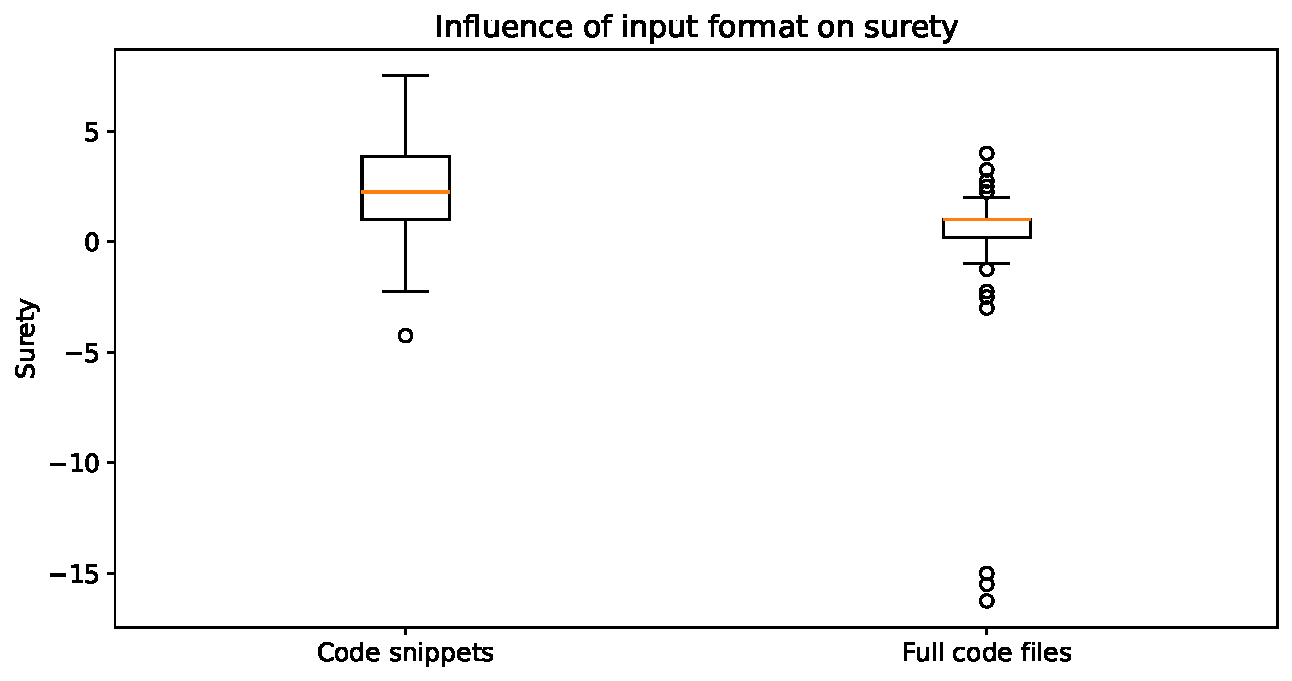
\includegraphics[width=\columnwidth]{figures/chapter5/detect_input_format_surety.pdf}
    \caption{Boxplot: Influence of input format on Surety}
    \label{fig:detect_input_surety}
\end{figure}

Analyzing the time needed to fulfill a request, it can be seen that some waiting time should be taken into account. The boxplot in figure \ref{fig:temperature_time} shows how the temperature of the model influences the processing time. The median time  decreases with increasing temperature. For instance, the median time for a temperature of 0.1 is nearly 100 seconds while it is nearly 50 seconds in the case a temperature of 0.9. Also, the upper whisker decreases from 250 to 150 while the lower whisker also decreases slightly. The existence of a multitude of outliers on the upper bound shows that the server response time can vary significantly. 

\begin{figure}
    \centering
    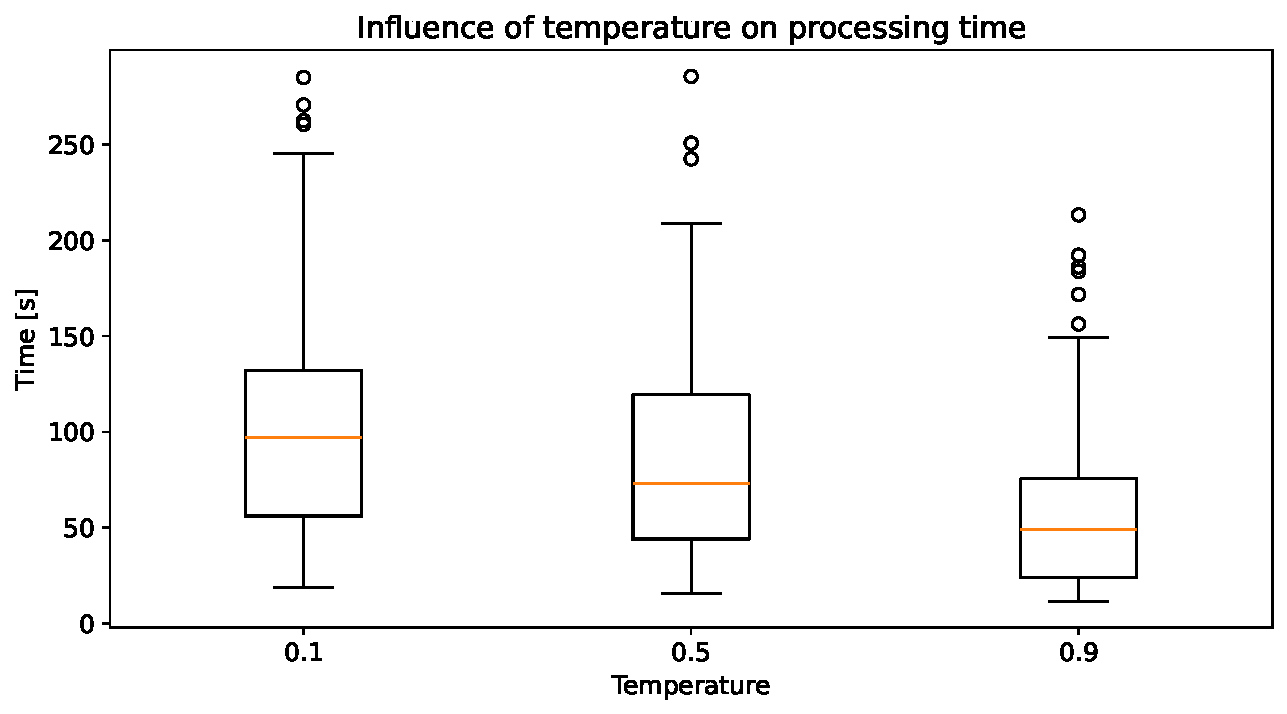
\includegraphics[width=\columnwidth]{figures/chapter5/detect_temperature_time.pdf}
    \caption{Boxplot: Influence of temperature on time}
    \label{fig:temperature_time}
\end{figure}

\subsubsection{Threats to validity}

In the detection experiment, the returned data clump type context is linked to the real data clump type context to determine which data clumps are detected. The metric finds the real data clump that shares the most similarities with the returned data clump. However, this could be a completely wrong data clump. For instance, if the model returns a correct class name containing a data clump but otherwise is wrong, it is still considered for the data clump type, size, and occurrence metric. The accuracy of the information is only considered in the surety metric.

Additionally for the output accuracy metric, the relevance of each parameter in data clump type context is disregarded. For instance, the data clump type context contains information about the line number of each data clump. Even if this information is missing, it can be replaced by considering the other information (variable names, method name, class name). 



\subsection{Experiment 2B: Data clump detection with modifications}

This experiment is a derivation from the preceding one. Similarly to the detection experiment, the goal is to detect data clumps in a software project.

However, now the source code is modified to test whether the model can detect data clumps that the \textit{DataClumpDoctor} would miss due to difference in the names or data types of the clump items. Three types of modification should be distinguished:

\begin{description}
    \item[Synonym:] A synonym of variable name is used. For instance, the words \textit{change} and \textit{modification} have a very similar  meaning. 

    \item[Typographical error:] A spelling error resulting in a slightly modified name. This could be caused by a developer not knowing the exact spelling of a word. However, it could also happen by accident if the developer mistypes while writing the source code.

    \item [Type mismatch:] Two variables that share the exact names but have a similar type .
\end{description}

In each of these cases, it can be argued that a data clump can still exist even with these modifications. For synonyms and type mismatches however, allowing such changes might increase the chance of false positives. 

\subsubsection{Methodology}

For this experiment, data clumps with exactly three items were randomly sampled. For each data clump, one modification was introduced (e.~g. replacing the name of a variables by a synonym), if such change was reasonable.

It is important to only consider data clumps with exactly three items because  a modification of one item would invalidate the data clump for a traditional tool like the \textit{DataClumpDoctor}. If larger data clumps were to be submitted, the model could return only a subset of the data clump items and ignore the item with the modifications. 

To find synonyms for a given word, the WordNet \cite{10.7551/mitpress/7287.001.0001} library was used. This library can find similar words to a given word.

To find typographical errors, the Birbeck database \cite{birbeck} was used which contains spelling mistakes in the English language. From this database, a spelling mistakes was chosen that could reasonably happen to a developer (e.~g. writing a letter twice, omitting a letter etc.). 

Type modifications were only performed on numerical types such as \textit{int}. For instance,  the type \textit{long} might be replaced by \textit{int}. 

The same metrics as in the detection experiment are used. Additionally, it is counted how often the model detects a data clump with a modification. 





\subsubsection{Results}

In summary, ChatGPT was able to detect data clumps with synonyms and typos while facing enormous challenges identifying data clumps with different types. However, the capability of ChatGPT ignoring such modifications varies strongly between projects. 

\begin{figure}[ht!]
    \centering
    \begin{subfigure}[t]{0.44\columnwidth}
        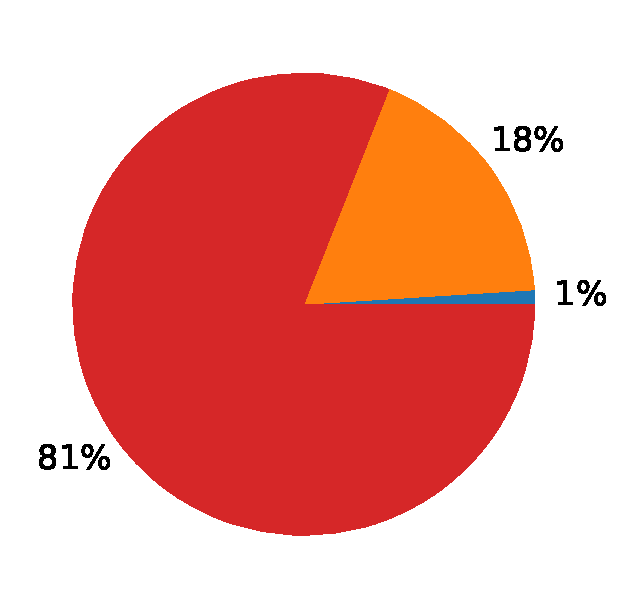
\includegraphics[width=0.8\columnwidth]{figures/chapter5/detectSyn_mod_type_argouml.pdf}
        \caption{ArgoUML}
        \label{fig:detect_syn_mod_type_argouml}
    \end{subfigure}
            \begin{subfigure}[t]{0.44\columnwidth}
        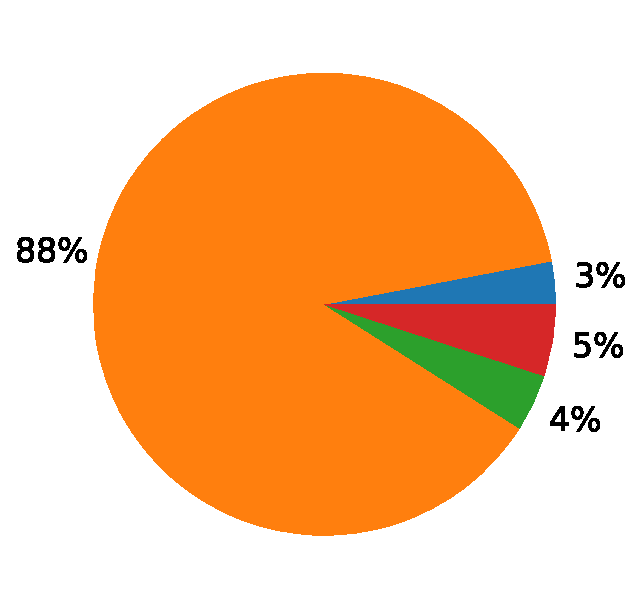
\includegraphics[width=0.8\columnwidth]{figures/chapter5/detectSyn_mod_type_rocketmq.pdf}
        \caption{RocketMQ}
       \label{fig:detect_syn_mod_type_rocketmq}
    \end{subfigure}
        \begin{subfigure}[t]{0.5\columnwidth}
        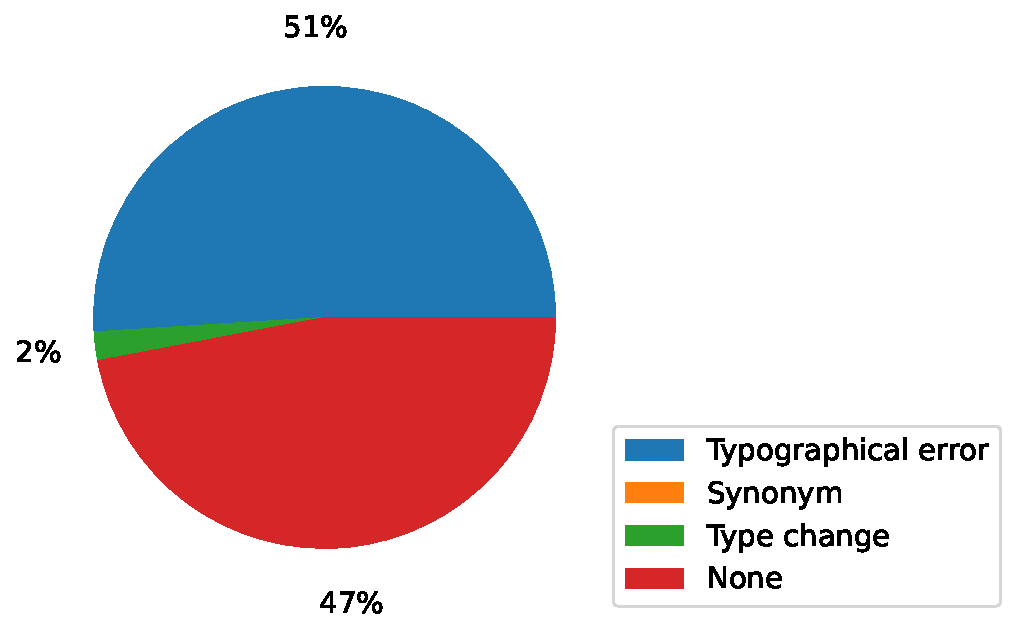
\includegraphics[width=1.2\columnwidth]{figures/chapter5/detectSyn_mod_type_dolphin.pdf}
        \caption{DolphinScheduler}
        \label{fig:detect_syn_mod_type_dolphinscheduler}
    \end{subfigure}

    \caption{Types of detected data clumps with modifications by project}
    
    \label{fig:detect_syn_mod_type}
\end{figure}


 The pie diagrams  \ref{fig:detect_syn_mod_type_argouml}, \ref{fig:detect_syn_mod_type_rocketmq}, and \ref{fig:detect_syn_mod_type_dolphinscheduler} depict the percentages of data clump detected by modification type. In the case of \textit{ArgoUML} and \textit{Dolphinscheduler}, 81~\% of the  data clumps detected were not modified. 18~\% of the detected data clumps have a synonym as a modification while the remaining 1~\% of the case belong the category data clumps with typos. No data clumps were detected that have a modified data type. 

 A stark contrast exists for \textit{RocketMQ}. 88~\% of the detected data clumps were modified by using a synonym. In 3~\% of the cases, the data clumps have a typo. A data type was modified in 4~\% of the identified data clumps. In the remaining 5~\%, the data clumps had no modifications. 

For \dolphinscheduler, the ratio of data clump with typos is 51~\% while in 47~\% of the identified data clumps no modifications were applied. In the remaining 2~\% of the cases, a data type was modified. No data clumps with synonyms were detected. 



The input format also has some influence on the category of data clumps detected. Figures \ref{fig:detectSyn_full_files} and \ref{fig:detectSyn_snippets} show the impact of the input format as a pie chart. 

 26~\% of the detected data clumps have a synonym as a modification if full code files are submitted. This value increases to 39~\% if code snippets are provided. On the hand, the percentage of detected data clumps with typos decreases from 21~\% to 17~\%. Also, the number of detected data clumps with data type modifications decreases from 4~\% to 1~\%. Consequently, 49~\% of the detected data clumps have no modifications if complete files are submitted while this value is 43~\% in the case of code snippets.  

\begin{figure}[ht!]
    \centering
    \begin{subfigure}[t]{0.5\columnwidth}
        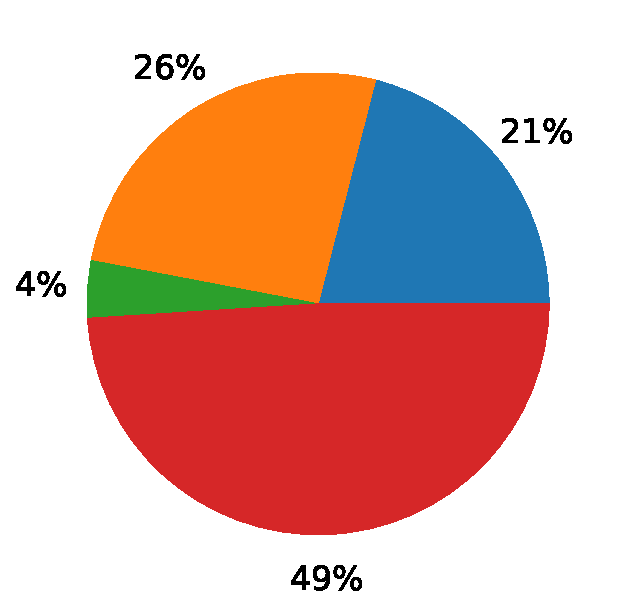
\includegraphics[width=0.8\columnwidth]{figures/chapter5/detectSyn_input_fullFile.pdf}
        \caption{Full code files}
        \label{fig:detectSyn_full_files}
    \end{subfigure}
            \begin{subfigure}[t]{0.5\columnwidth}
        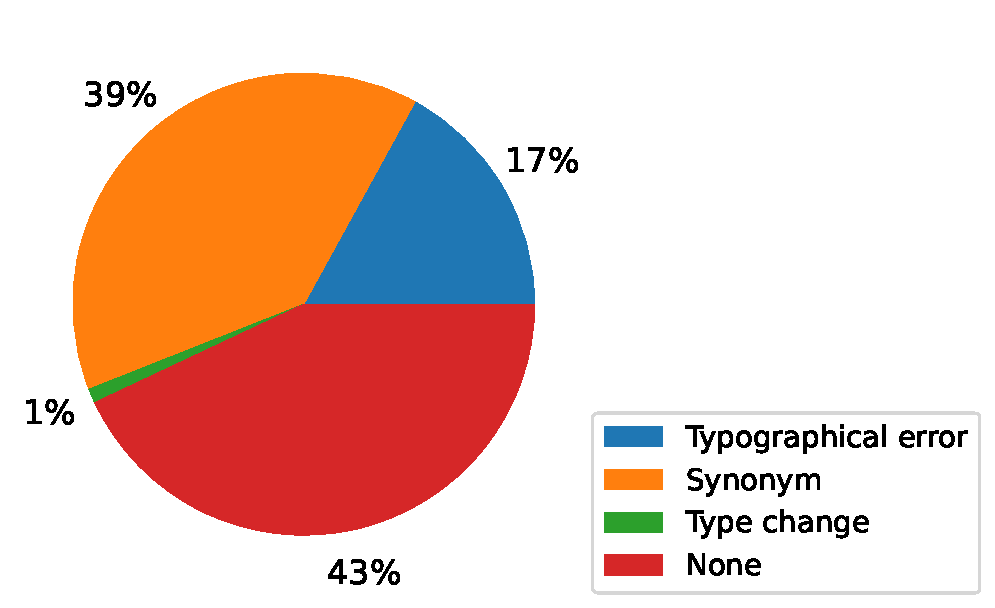
\includegraphics[width=1.3\columnwidth]{figures/chapter5/detectSyn_input_snippet.pdf}
        \caption{Code snippets}
       \label{fig:detectSyn_snippets}
    \end{subfigure}
       

    \caption{Types of detected data clumps with modifications by input format}
    
    \label{fig:detect_syn_input_type}
\end{figure}

\subsubsection{Threats to validity}
In general, the Threats to validity from the detection experiment apply here too. 

Additionally, the concrete modification applied to a data clump item can strongly affect the result. For instance, the Birbeck dataset contains mostly spelling mistakes made by children or illiterate adults so that developers could possibly make other mistakes which would be easier to spot for a model. 

Also the WordNet database is not specialized on technical terms but is more general. This means that the synonyms chosen here might not be synonyms used by a developer.

\subsection{Experiment 2C: Data clump filtering by model}

The filtering experiment is somewhat similar to the detection experiment. However, here the model is told to return one data clump that is most relevant. Additionally, it does not need to use the data clump type context as the output format because this information already exists. 

As outlined in section \ref{sec:data_clump_filtering}, there are multiple approaches for filtering data clumps, which can already be implemented manually. 
The question here is whether the \ac{LLM} uses novel filtering approaches or simply relies on the metric discussed in section \ref{sec:data_clump_filtering}. In the latter case, it is more useful to use the manual algorithm because they are reliable and do not incur the costs associated with Large Language Models. 

\subsubsection{Methodology}

This experiment is conducted similarly to the detection test. However, at this time, the data clump type context as outlined in appendix \ref{app:data_clump_format} is included as a possible input format. Additionally, if code snippets are provided, they always contain data clumps as opposed to possible data clumps as outlined in the detection experiment. 
The output format is discussed in section \ref{sec:output_format_filtering}
The following metrics are used to evaluate this experiment:
\begin{description}
    

    \item [Surety:] This metric is identical to the surety metric in the detection experiment. 
    \item [Reason:] A reason given by the model that explains why the model chose a particular data clump. 
    \item [Position on ground truth:] The minimal index of the data clump with respect to the occurrence, size, and affected files metrics.
\end{description}


\subsubsection{Results}

Figures \ref{fig:filter_reason_argouml}, \ref{fig:filter_reason_rocketmq}, and \ref{fig:filter_reason_dolphinscheduler} visualize the distribution of the reason provided by the model as a pie diagram.

For \argouml, in 42~\% of the cases, the model named the number of affected files as the reason to return a specific data clump. In 15~\% of the cases, the size of the data clump was the most important factor. The occurrence mattered in 13~\% of the cases. In the remaining 30~\% of the cases, the \ac{LLM} chose the data clump because of the domain of the variables. 

Considering the project \rocketmq, it can be seen that the percentage of the reason \enquote{Affected files} is also relatively large with 33~\%. Additionally, the occurrence was mentioned in 38~\% of the cases. In 19~\% of the filtering proposals, the size of the data clump was named as the reason for refactoring. Lastly, the domain of the data clump variables was specified as the model's choice in 10~\% of the cases.

In the case of \dolphinscheduler, the importance of the domain is greater since 36~\% of the suggestions named this reason. Additionally, the affected files played a less role as the percentage is 14~\%. The same applies to the reason \enquote{size} which is 4~\%. On the other hand, the occurrence of the data clump remained an important reason for the model as it was named in 46~\% of the cases. 
\begin{figure}[ht!]
    \centering
    \begin{subfigure}[t]{0.48\columnwidth}
        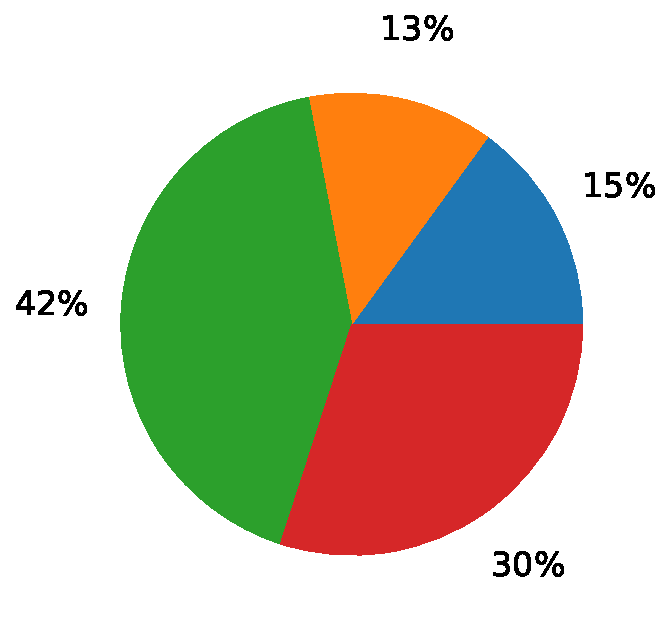
\includegraphics[width=1\columnwidth]{figures/chapter5/filter_reason_argouml.pdf}
        \caption{ArgoUML}
        \label{fig:filter_reason_argouml}
    \end{subfigure}
            \begin{subfigure}[t]{0.48\columnwidth}
        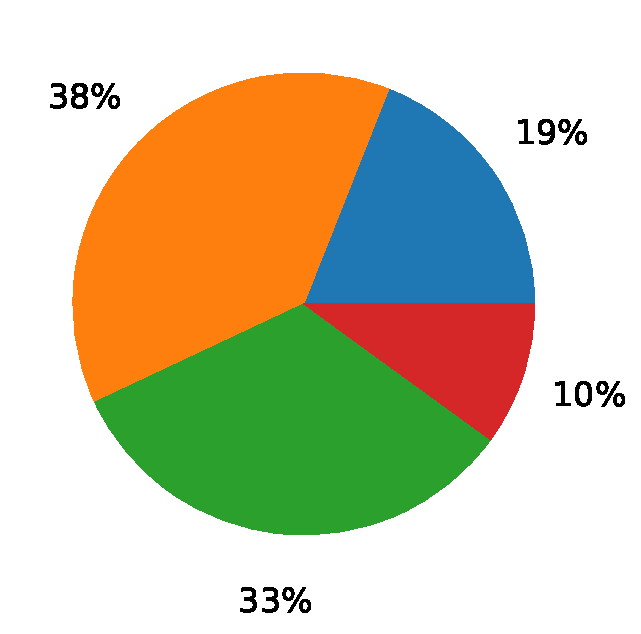
\includegraphics[width=1\columnwidth]{figures/chapter5/filter_reason_type_rocketmq.pdf}
        \caption{RocketMQ}
       \label{fig:filter_reason_rocketmq}
    \end{subfigure}
        \begin{subfigure}[t]{0.6\columnwidth}
        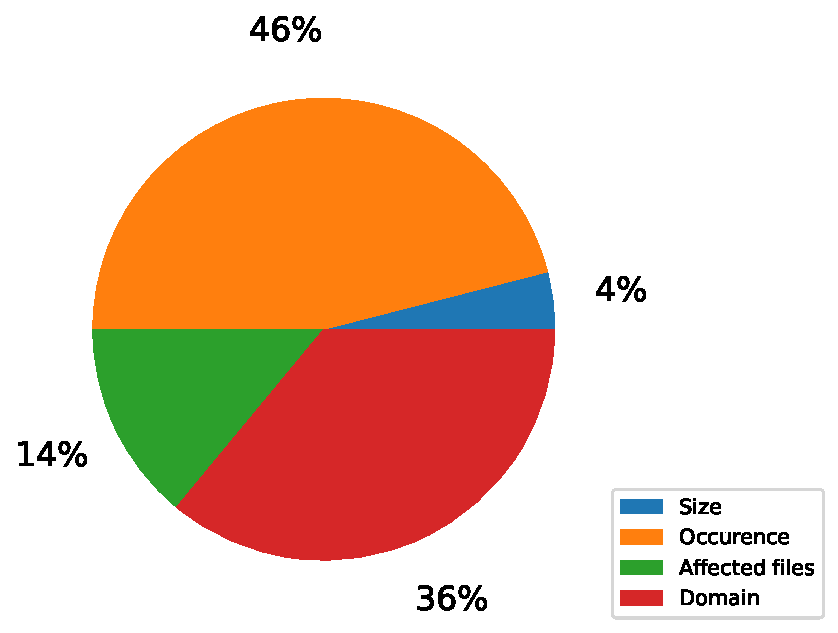
\includegraphics[width=1.3\columnwidth]{figures/chapter5/filter_reason_type_dolphin.pdf}
        \caption{DolphinScheduler}
        \label{fig:filter_reason_dolphinscheduler}
    \end{subfigure}

    \caption{Distributions of reasons for selecting a data clump provided by the model }
    
    \label{fig:filter_reason}
\end{figure}

The position on the ground truth varied per project. The box plot in figure \ref{fig:filter_project_posgroundtruth} visualizes the distribution.  

For \argouml, the median is zero and no whiskers  are visible. However, a multitude of outliers up to 12 are present. This means that in most cases, the model chose the same data clump as a traditional metric. 

On the other hand, \rocketmq shows that the model could choose other data clumps. Here, the lower whisker is 0 while the upper whisker is  3, The median is 2 meaning that the model more often returned a data clump that a traditional algorithm would not suggest.

For \dolphinscheduler, the median is also 2 though in this case no whiskers are visible. This indicates that here also the model would return data clumps more difficult to detect via a classical algorithm. 
\begin{figure}
    \centering
    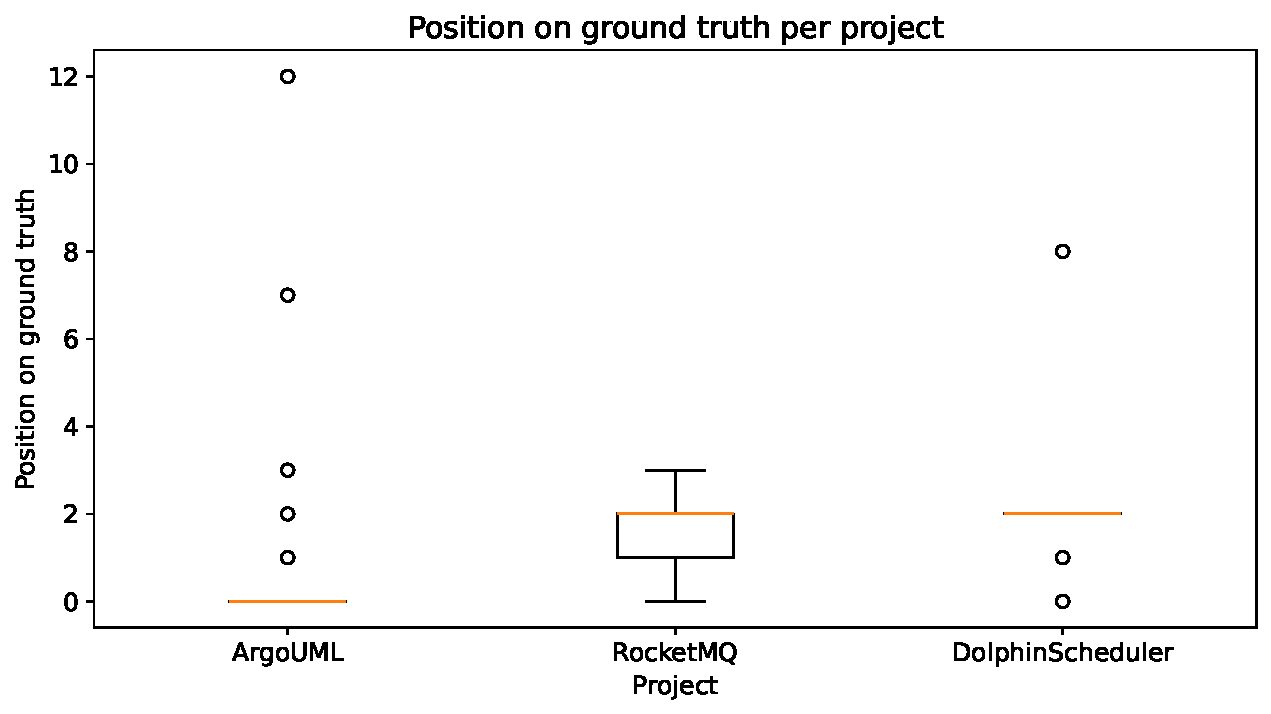
\includegraphics[width=\columnwidth]{figures/chapter5/filter_project_position_groundtruth.pdf}
    \caption{Position on ground per project}
    \label{fig:filter_project_posgroundtruth}
\end{figure}


\subsubsection{Threats to validity}

One threat of validity is   that only one data clumps is returned although it might make sense to return more (e.~g. three). Additionally, as a result of the similarity to the detection experiment, the flaws of the former can be flaws of the latter experiment. 

Moreover, the reason returned by the model should be taken with a grain of salt. The model might claim that is chooses a specific data clump because of its domain but in truth it might have applied other criteria. Hence,  is impossible to verify the reason


\subsection{Experiment 2D: Data clump refactoring}

Evaluating how an \ac{LLM} performs data clump refactoring is another method to assess the suitability of the models for use in the pipeline. Here, especially the creativity is important. If a model merely refactors similarly to a manual tool (e.~g. IntelliJ), it has less use.

If, however, the \ac{LLM} extracts more functionality by creating new methods or solves the data clump in other ways, the advantages of the model become more obvious.



\subsubsection{Methodology}

In contrast, to the detection and filtering experiment, this experiment included actual modification to the source code. 

The model is instructed to find and refactor all data clumps. 
The model outputs by providing diff instruction as discussed in section \ref{sec:output_processing} and the modifications are applied.  The modified program is tested with the respective build system (Gradle or Maven). If the build fails, the model is provided with error messages and the content of the affected lines, and the model is instructed to fix these issues. If after five attempts, the project still does not compiles, no further attempts are made. 

The following metrics are used for evaluating this test:

\begin{description}
    \item [Compilation attempts:] The number of attempts remaining. For instance, if the model takes four iterations to fix all compilation issues, one iteration is remaining. 
    \item[Final program validity:] Whether a refactored program is compilable at the end. 
   \item [Reference error ratio:] This metric shows the ratio of reference errors over all compiler errors. Reference errors are errors about unknown methods, variables etc.  A reference error can be described as  a \enquote{good} error because it could be fixed more easily. On the other hand, a syntactical error like missing parentheses or non-closed comments are more difficult to handle. 
    \item [Rich class:] Whether the extracted class are more than mere data classes
   
    \item [Removed data clumps:] This metric assesses how many data clumps were removed during the refactoring process

    \item [Removed variables:] In contrast to the removed data clump metric, this metric counts the total number of fields and parameters removed during the refactoring process even if these removals do not lead to less data clumps, 
\end{description}



\subsubsection{Results}

In general, ChatGPT is unable to fully perform the refactoring so that the resulting program does compile and work. However it is able to remove many variables and decrease the code size. Many refactorings however are incomplete so that the data clump still remains partly. 

In about 40 percent of the instances, ChatGPT fails to provide concrete diff instructions which means that the source code cannot be changed given the information provided by the model. This indicates that while the diff instructions are helpful to ease refactoring, the model is not trained enough to fully use their potential. 

Additionally, the extracted class are seldom rich (10 percent) which indicates that generating helpful classes is possible but still limited. 
\begin{figure}
    \centering
    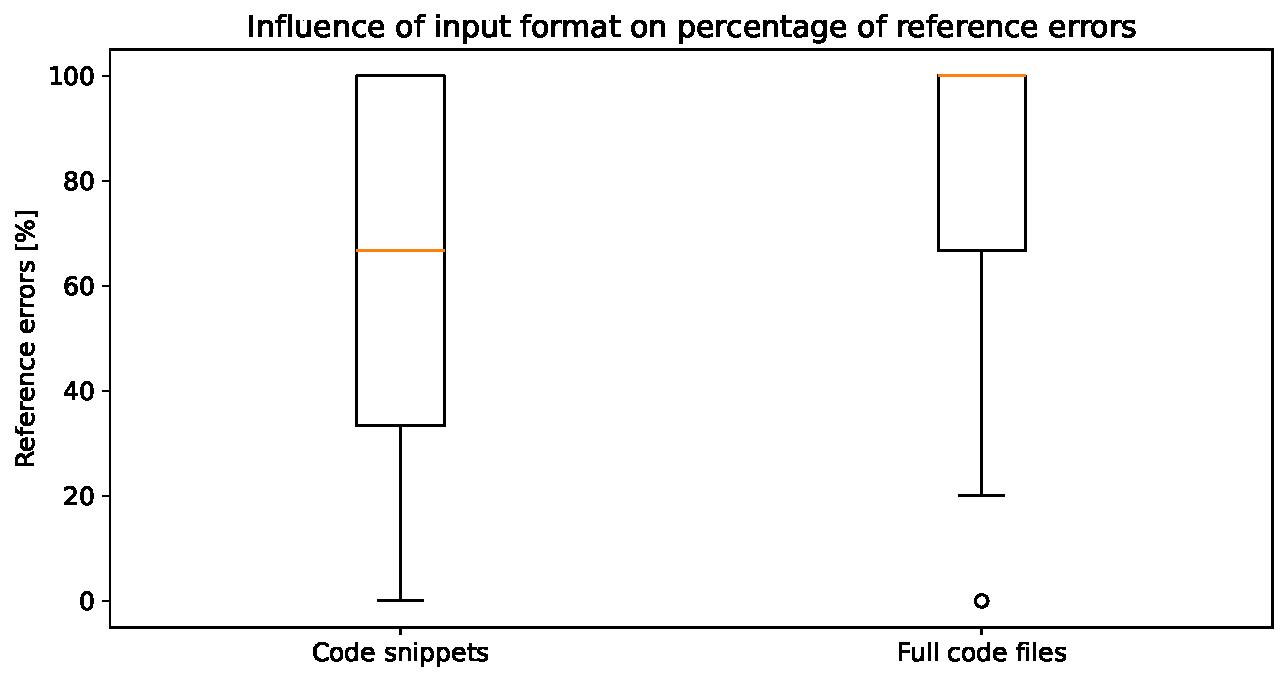
\includegraphics[width=\columnwidth]{figures/chapter5/refactor_input_referenceerrors.pdf}
    \caption{Proportion of reference errors on all errors by input format}
    \label{fig:refactor_input_referenceerrors}
\end{figure}




Additionally, the effect of the input type is visible. Providing full code files decreases the number of valid diff instructions and leads to less removed variables.  Additionally, as figure \ref{fig:refactor_input_referenceerrors} depicts, the complete source code approach leads to less syntactical errors but more errors related to non-updated references (e.~g. method calls).  The left box plot shows a median of about 65~\% and a lower whisker of 0~\% while an upper whisker is not visible. If code snippets are provided, the median increases to 100~\% indicating that syntactical errors are less common. However, the lower whisker is 20~\% which means that such errors can still occur. The outlier at 0~\% further shows that even providing full code files did not prevent major syntactical errors. 


This shows that the snippet approach is not well-handled by the model as it more often introduces syntax errors. 



As for the margin parameters, there is a strong contrast between a margin of 0 and larger margins. For instance, a margin of 0 leads to a high number of non-interpretable diff instructions. Here also, many results are inconclusive and vary between projects. 

Higher margins also led to a decrease in the number of removed data clumps as the box plot in figure \ref{fig:refactor_margin_removedDataClumps} shows. 
For a margin of 0, there is a greater variance. The median is 1 while the upper whisker is nearly 6. The lower whisker is 0. A margin of 1 decreases the median number of removed data clumps and also the value of the upper whisker to about 3. A similar decrease happens if the margin is increased to 2. If the margin is 5 or 10, median becomes 0 while the upper whisker is close to 1. For all margins larger than 0 a significant amount of outliers are present indicating that while data clumps were removed seldom, there were instances where the removal was successful. 
\begin{figure}
    \centering
    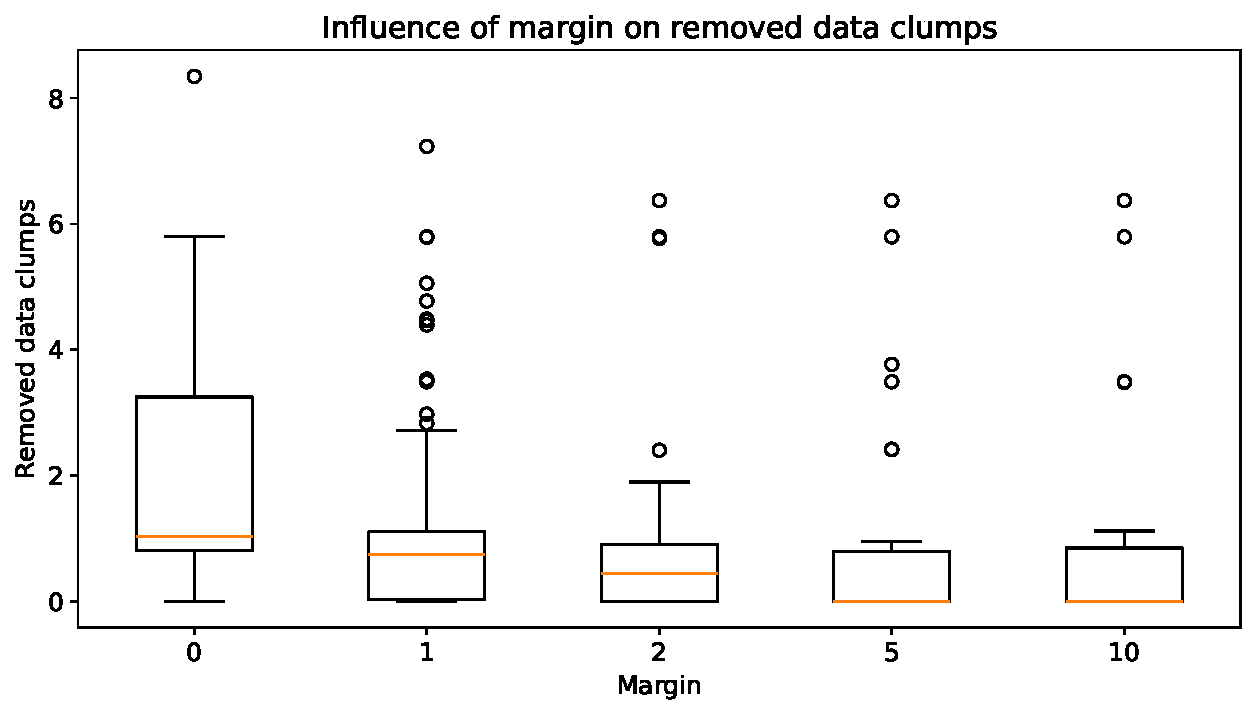
\includegraphics[width=\columnwidth]{figures/chapter5/refactor_margin_removed_data_clumps.pdf}
    \caption{Box plot: Influence of margin on removed data clumps}
    \label{fig:refactor_margin_removedDataClumps}
\end{figure}

\subsubsection{Threats to validity}

For the refactoring experiments, several limitation should be considered. Noteworthy, the number of data clumps transmitted is severely limited as the model should also correct errors which requires retransmitting files multiple times. In many cases, this repeated transmission can exceed the context window so that the number of data clumps (and hence in most cases the number of transmitted files)  needs to be reduced. 

Additionally, in the validation phase, the instruction to fix errors is constant, namely \enquote{Fix all errors in the respective files}. In contrast to a human in the loop who might be able to help the model to solve the compiler errors, the model can only rely on the compiler errors and the content of the files affected by these compiler errors. This can be problematic if the model returns a specific correction output but this output cannot be parsed correctly (e.~g. wrong line numbers). In that case, no compiler errors are fixed and the model might be tempted to use the same output again until the five attempts are exhausted. This problem could only be prevented if concrete feedback is given which is outside of the scope of this master's thesis. 

\subsection{Discussion}



The results from all four experiments show that ChatGPT has potential to be used in the pipeline but many challenges still exists.

As outlined in experiment 2A, The model is capable of detecting some data clumps but due to output size limitation, the number of data clumps is limited. However, the limited number of data clumps might also be a sign of filtering so that non-important data clumps are ignored.

Experiment 2B shows that the model can also detect data clumps that a tool like the \textit{DataClumpDoctor} would not be able to detect. This is useful as a single typo can invalidate a data clump relationship so that a traditional tool would not be able to detect this data clump. This also applies to synonym although one must be cautious as the risk of false positive is higher.

The filtering experiment 2C illustrates that ChatGPT can also find a suitable data clump for refactoring given they have been already detected. This data clump is not always the one proposed by a traditional metric so that other reasons than size or occurrence are used to make a decision on what data clump to refactor. However, as the first experiment shows, the data clump proposed might not be a data clump that a developer wants to refactor. As a result, further investigations about the reasons developer would like to remove data clumps for are warranted.

As for the last experiment 2D,  challenges are clearly visible. While data clumps can be removed by the model, the programs refactored are mostly non-compilable. Additionally, the model is unable to fix those errors which means a human-in-the-loop must intervene. Therefore, automatic data clump refactoring via \acp{LLM} is only imaginable if the model only performs tasks that do not change the source code. A traditional tool like an IntelliJ plugin can then perform the refactoring as it is reliable. 


As to RQ 3, the effect of the parameters can have a significant influence on the quality of the results.  For instance, the code snippet approach is suitable for detecting data clumps while increasing the potential of hard-to-fix errors if it is used for refactoring.
However, other parameters like the margin or temperature do not have a consistent effect on the performance of the model. Hence, practitioners should generate multiple proposals using multiple parameters and  select a suitable one (manually or automatically). This underscores that \acp{LLM} do not always give the best response at first, and comparing multiple solution to a problem (e.~g. multiple data clump refactoring proposals) is one key to improve the integration of \acp{LLM}. 

Further experiments needs to be conducted that analyze the stark difference of parameter's impact on the quality of the results. The observations discussed in  \cite{hallCodeSmellsHave2014} shows a similar discrepancy with regard to data clumps per projects although there it is about the induction of faults.

In summary, it is evident that ChatGPT has some strengths if used in the pipeline which can only hardly be replaced by traditional tools.   For instance, it does not always return the same data clump (e.~g. largest) but uses other metrics in contrast to an approach via classical filters. However, there are many challenges that prevents an fully autonomous refactoring via ChatGPT. 





